\documentclass[10pt]{article}
\usepackage{graphicx}
\usepackage[margin=1in]{geometry}
\usepackage{titlesec}
\usepackage{multicol}
\usepackage{multirow}
\begin{document}
\begin{center}
\Large{Parcial 1 - Optimizaci\'on}

\Large{Gerardo Andr\'es Ria\~no Brice\~no - 201112388}
\medskip
\hrule
\end{center}

\setlength\parindent{0pt} 

{\bf \Large{Problema 1}}
\medskip

En principio, es clave identificar que la variable $x_3$ es libre es decir $x_3\leq0$ y $x_3\geq0$ y se encuentra dentro de la funci\'on de costo con coeficiente diferente de cero. Por lo cual, es necesario realizar modificaciones con variables auxiliares para que el programa lineal quede en la forma est\'andar y sea posible obtener la primera soluci\'on b\'asica factible. Adicionalmente, como el tipo de restricciones es el mismo, de mayor o igual, al incluir variables de holgura se obtendr\'a la primera soluci\'on b\'asica factible, sin necesidad de resolver un problema auxiliar de la forma $1^Ty$. \\

Se hace un cambio de variables $x_3 = y_1-y_2$ con $y_1, y_2 \geq 0$. De esta forma, se sigue cumpliendo que $x_3$ es libre dado que, $y_1>y_2\rightarrow x_3\geq0$ y $y_1<y_2\rightarrow x_3\leq0$

Ahora bien, se utilizan variables de surplus, dado que las desigualdades son de la forma $\geq$ y se obtiene el programa est\'andar de la forma:

\begin{center}
\[\min_{x,y}  3x_1+4x_2+2(y_1-y_2)\] 

sujeto a

$-4x_1+8x_2+2y_1-2y_2-k_1 = 20$

$2x_1-4x_2+y_1-y_2-k_2 = 12$

$2x_1+12x_2+4y_1-4y_2-k_3 = 16$

$x_1, x_2, y_1, y_2, k_1, k_2, k_3 \geq 0$

\end{center}

Con el programa lineal en la forma est\'andar se forma el Tableau que lo representa y se multiplican las restricciones de igualdad a ambos lados por -1 para obtener la identidad, i.e. la base del sistema lineal.

\begin{center}
\begin{tabular}{c c c c c c c |c}
$x_1$&	$x_2$&	$y_1$&	$y_2$&	$k_1$&	$k_2$&	$k_3$&b\\	
4	&-8&	-2&	2&	1&	0&	0&	-20 \\
-2&	4&	-1&	1&	0	&1&	0&	-12 \\
-2&	-12&	-4&	4&	0	&0&	1&	-16 \\
\hline
3&	4&	2&	-2&	0&	0&	0&	0\\
\end{tabular}
\end{center}

Se tiene entonces que la primera soluci\'on b\'asica factible del programa lineal es $x_1=x_2=y_1=y_2=0$, $k_1=-20$, $k_2=-12$ y $k_3=-16$. \\

1b) La soluci\'on no es \'optima, dado que el valor de uno de los costos reducidos es negativo $r_4$.

\bigskip
{\bf \Large{Problema 2}}
\medskip


Problema primal:

\begin{center}
\[\min_{x}  4x_1+6x_2+2x_3+6x_4+2x_5\] 

sujeto a

$2x_2-2x_3-2x_4+2x_5 = -5$

$-x_1-x_2+x_3-x_4+x_5 <= 2$

$x1, x2, x3, x4, x5 >= 0$

\end{center}

Se obtiene el programa dual con base en las reglas de conversión descritas en la tabla de Tucker. \\


Problema dual:
\begin{center}
\[\max_{\lambda} -5\lambda_1+2\lambda_2 \] 

sujeto a

$-\lambda_2 \leq 4$

$2-\lambda_2\leq6$

$-2+\lambda_1\leq2$

$-2-\lambda_2\leq6$

$2-\lambda_2\leq2$

$\lambda_2\geq0$

\end{center}

\begin{figure}[ht!]
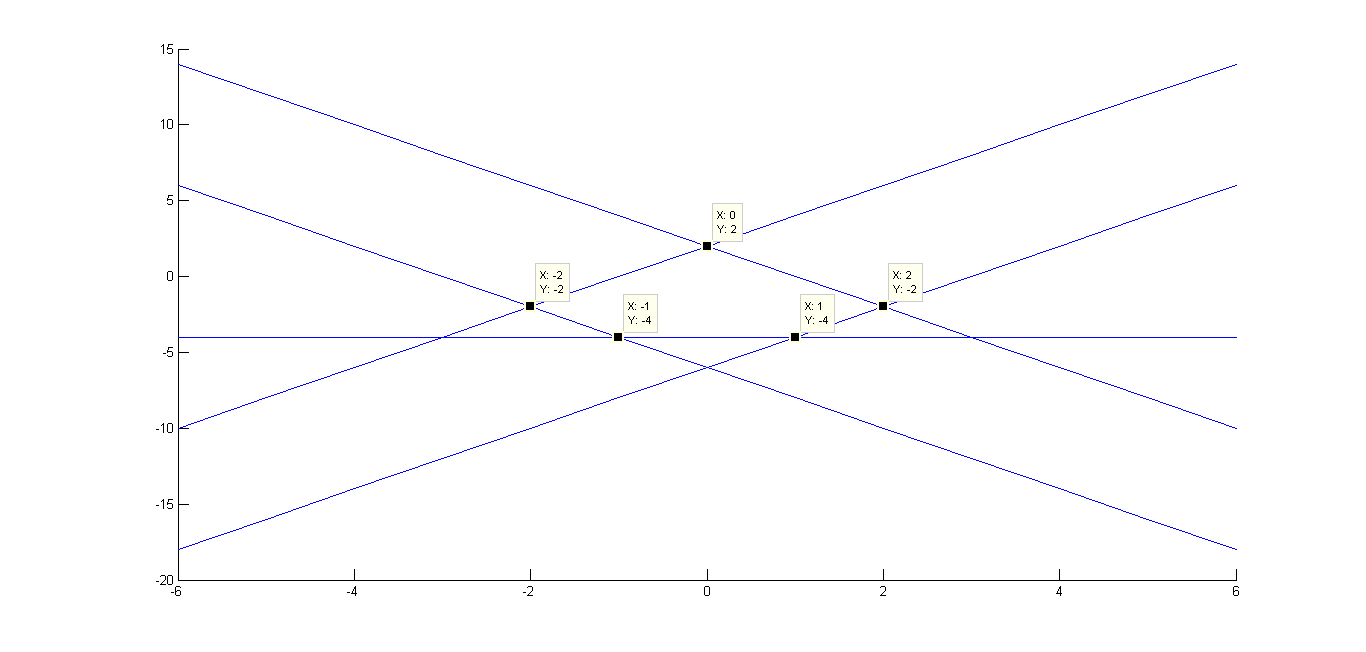
\includegraphics[width=160mm]{factible.png}
\end{figure}

Ahora, se grafican las restricciones para el dual y se identifican gr\'aficamente las soluciones básicas factibles del PL. Con estas soluciones se eval\'ua la funci\'on de costo y se escogen los $x_1$ y $x_2$ que aseguran un valor \'optimo para el dual.
\bigskip

\begin{center}
\begin{tabular}{c c c}
{\bf$\lambda_1$}	& {\bf$\lambda_2$} &{\bf$fcosto$} \\
0&	2&	4\\
2&	-2&	-14\\
1&	-4&	-13\\
-1&	-4&	-3\\
-2&	-2&	6\\
\end{tabular}
\end{center}

La soluci\'on para el dual es $\lambda_1 = \lambda_2 = -2$.
\bigskip

2b) En principio, se determinan las soluciones activas en el dual.

\begin{center}
$2	\leq	4$ \\
$-2	\leq	6$ \\
$2	\leq	2 \rightarrow$ Soluci\'on activa\\
$6	\leq	6 \rightarrow$ Soluci\'on activa \\
$-6	\leq	2$ \\

\end{center}


Dado que las restricciones 3 y 4 son soluciones activas, por holgura complementaria $x_1, x_2 y x_5$ son iguales a cero y debe cumplirse que:

\begin{center}
$2x_3+	6x_4 =	6$ \\
$-2x_3	-2x_4=-5$ \\
$x_3	-x_4 =	2$\\

\end{center}

La primera ecuaci\'on es combinaci\'on lineal de las otras dos, por lo cual se puede resolver el sistema de ecuaciones quitando una ecuaci\'on. Como soluci\'on se obtiene que $x_3=9/4$ y $x_4=1/4$.

Por lo tanto, la soluci\'on \'optima para el primal es: \\
\begin{center}
$x_1=0, x_2=0, x_3=9/4, x_4=1/4, x_5=0$

\end{center}

y la soluci\'on \'optima para el dual,

\begin{center}
$\lambda_1=-2, \lambda_2=-2$
\end{center}

{\bf \Large{Problema 3}}
\medskip

El problema de maximizaci\'on es equivalente al de minimizaci\'on de $-f(x)$.

\begin{center}
\[\min_{E,M,S} -60E-30M-20S \] 

sujeto a

$8E+6M+S\leq48$ \\
$4E+2M+1.5S\leq20$ \\
$2E+1.5M+0.5S\leq8$ \\
$E, M, S \geq 0$
\end{center}

3b) Se utiliza el m\'etodo Simplex revisado dado que facilita el c\'alculo de los multiplicadores Simplex. Se utilizan variables de holgura $y_1$, $y_2$, $y_3 \geq0$ para poner el problema en la forma est\'andar.


\begin{center}
\begin{tabular}{c c c c c c |c}
E  & M   & S   & $y_1$&	$y_2$&$y_3$&b\\	
8  & 6   & 1   & 1 & 0 & 0 & 48 \\
4  & 2   & 1.5 & 0 & 1 & 0 & 20 \\
2  & 1.5 & 0.5 & 0 & 0 & 1 & 8 \\
\hline
-60 & -30  & -20  & 0 & 0 & 0 & 0 \\
\end{tabular}
\end{center}

Los pasos del proceso del Simplex revisado se mostrar\'an siguiendo la forma de Tableau que se muestra a continuaci\'on.

\begin{center}
\begin{tabular}{c|c}
B & Nb\\	
\hline
$C_b$ & $C_n$\\
\end{tabular}
\end{center}

Primera iteraci\'on, $r=[-60,-30,-20,0]$

\begin{center}
\begin{tabular}{c c c | c c c c}
1	&0	&0&			8	&6	&1	&48\\
0	&1	&0	&		4	&2	&1.5&	20\\
0	&0	&1	&		2	&1.5&	0.5&	8\\
\hline							
								
0	&0&	0&			-60	&-30&	-20&	0\\
\end{tabular}
\end{center}

Segunda iteraci\'on, $r=[30, 15, -5, 240]$

\begin{center}
\begin{tabular}{c c c | c c c c}
1	&0	&8&			0	&6&	1	&48\\
0	&1	&4	&		0	&2	&1.5&	20\\
0	&0&	2	&		1	&1.5&	0.5&	8\\
								
								
0&	0&	-60		&	0&	-30&	-20	&0\\
\hline							
								
0	&0&	0&			-60	&-30&	-20&	0\\
\end{tabular}
\end{center}

Tercera iteraci\'on, $r=[10, 5, 10, 280]$

\begin{center}
\begin{tabular}{c c c | c c c c}
1&	1	&8		&	0&	6	&0&	48\\
0&	1.5	&4		&	0&	2	&1	&20\\
0&	0.5	&2		&	1&	1.5&0&	8\\
								
								
0&	-20&	-60		&	0	&-30&	0&	0\\
\end{tabular}
\end{center}

\begin{center}
$x_B = [24,8, 2]$\\
$\lambda = c_B \cdot B^{-1}$\\
$\lambda = [0, -10, -10]$\\
\end{center}

3c) Es importante tener en cuenta que los multiplicadores simplex est\'an relacionados con el costo sint\'etico. Ahora bien, un costo razonable es aquel con el cual el costo reducido no sea menor a cero, i.e. con el cual no sea necesario gastar m\'as de lo que se gasta con el \'optimo. Se calculan el nuevo costo reducido:

$r=c_b- \lambda^T[1, 0.3, 0.5]$
$r=c_b-(-8)$
 
El costo de los bancos debe ser menor o igual a 8.


\end{document}
